\documentclass{beamer}

\usepackage{amssymb,amsmath,verbatim,graphicx,microtype,units,booktabs,upquote,xcolor,siunitx,csquotes,fancyvrb,newverbs,wrapfig,multicol,tikz,textcomp}
\usepackage{fontawesome,setspace} % ONLY BUILD WITH XELATEX
\usetikzlibrary{arrows,automata,positioning}
\hypersetup{
            colorlinks = true,
            linkcolor = blue,
            urlcolor  = blue,
            citecolor = blue,
            anchorcolor = blue
}

\title{Fundamentals of Git}
\subtitle{Missouri Satellite Team}
\author{Presented by: Illya Starikov}
\date{ }

\newcounter{branching}
\newcounter{committing}
\newcounter{merging}
\newcounter{conflicts}

\newcommand{\shellcmd}[1]{\texttt{\colorbox{gray!30}{#1}}}
\newcommand{\presentcount}[1]{\addtocounter{#1}{1}\Roman{#1}}

\definecolor{cverbbg}{gray}{.7}
\newenvironment{lcverbatim}
 {\SaveVerbatim{cverb}}
 {\endSaveVerbatim
  \flushleft\fboxrule=0pt\fboxsep=.5em
  \scriptsize
  \colorbox{cverbbg}{%
    \makebox[\dimexpr\linewidth-2\fboxsep][l]{\BUseVerbatim{cverb}}%
  }
  \endflushleft
}

\newcommand{\hugeslide}[1]{
\begin{frame}[plain,c]
    \centering {\usebeamerfont*{frametitle} \usebeamercolor[fg]{frametitle}\fontsize{40}{50}\selectfont \textit{#1}}
\end{frame}
}
\begin{document}
\begin{frame}
    \maketitle
\end{frame}

\begin{frame}
    \frametitle{Getting Started}

    There'll be some setting up before you can start using git. It'll depend on your operating system --- you can refer to the installation guide
    \href{https://git-scm.com/book/en/v2/Getting-Started-Installing-Git}{here}.
    Below are the more popular methods of installation.

    \begin{description}
        \item[macOS] \shellcmd{brew install git}\footnote{Or whatever hip package manager you use.} or installing \href{http://osxdaily.com/2014/02/12/install-command-line-tools-mac-os-x/}{command lines tools}.
        \item[Linux] Depends on your distro. If Ubuntu use \shellcmd{sudo apt-get install git-all}, if Arch Linux then \shellcmd{pacman -S git}, if others refer \href{https://git-scm.com/download/linux}{here}.
        \item[Windows] Download a \texttt{.exe} from \href{https://git-scm.com/download/win}{here}.
    \end{description}

\end{frame}

\begin{frame}
    \frametitle{Getting Started}
    If you would like to follow along, navigate to \url{https://github.com/IllyaStarikov} \textrightarrow \ repositories \textrightarrow \ msat-git-tutorial \textrightarrow \ clone or download\footnote{
\includegraphics[width=0.5\textwidth]{github-clone}}. From here, you can either download as you normally would, or you use the super-cool terminal way:

    \begin{enumerate}
        \item Copy the link provided (something like \url{https://github.com/IllyaStarikov/msat-git-tutorial.git}).
        \item Open your terminal emulator of choice.
        \item Navigate to desired directory (using \shellcmd{cd DIRECTORY})
        \item Type in \shellcmd{git clone LINK}, where link is the copied link from Step \#1.
    \end{enumerate}


\end{frame}

\begin{frame}
    \frametitle{What is Git?}

    \begin{multicols}{2}
        \begin{itemize}
            \item Git is nothing more than Directed Acyclic Graph of objects compressed and identified by an SHA-1 hash. % What?
            \item Git works in snapshots, not differences. % Meaning when you commit (or save), you save a mini filesystem at the time of commit. This makes going through and seeing changes very easy
                \item Git is local. % Changes can be saved and continue your work no matter where you are. You can't receive/transmit changes from the remote, central repository, but you can continue your work (when you are ready to pull changes from central repo, it'll merge).
            \item Git has data integrity. % That's the SHA-1 hash. All your snapshots are referred to by a checksum.
            \item Git is parallelizable. % Meaning hundreds of people can work on hundreds different versions of the repository, and it'll still work.
        \end{itemize}

        \begin{center}
            
\includegraphics[width=0.35\textwidth]{xkcd}
        \end{center}
    \end{multicols}
\end{frame}

\begin{frame}
    \frametitle{The Five Stages of Git}

    \begin{enumerate}
        \item Working Directory % This is the local repository. The changes and modification you make are in this stage, until you 'add' (i.e. specifically say these are the files whos changes you want to `commit') them.
        \item Staging Area % When files are 'added', they are in the staging area, you ready for you to say `these are the changes I made'.
        \item Git Directory % After `committing' (nothing more than saying I made these changes, here's what's different), they are updated in the git databases
        \item $\cdots$
        \item Profit % fuck yeah!
    \end{enumerate}
\end{frame}

\begin{frame}
    \frametitle{\shellcmd{Git}ting Good}

    If the ``stages'' didn't make sense, that's alright. It's better to go through a workflow apposed to the formalities.

    \begin{enumerate}
        \item Start a new repository with \shellcmd{git init} % this creates your working directory
        \item Work on project in bite sized chunks, and add files that were changed with \shellcmd{git add file(s)} % adding to the staging area
        \item Commit your changes with \shellcmd{git commit} % This transfers them to the Git directory
        \item $\cdots$
        \item Profit.
    \end{enumerate}
\end{frame}

\begin{frame}
    \frametitle{Committing \presentcount{committing}}
    \only<1>{\shellcmd{git commit -m ``a''}}
	\only<2>{\shellcmd{git commit -m ``b''}}
	\only<3>{\shellcmd{git commit -m ``c''}}

    \vfill
	\centering
	\begin{tikzpicture}[->,>=stealth',shorten >=1pt,auto,node distance=2cm,
		semithick]
		\tikzstyle{every state}=[node distance=1.5cm]

		\node[state]   (A)  {a};

		\only<2->{%
			\node[state] (B) [below of=A] {b};
			\path (A) edge (B);
		}

		\only<3->{%
			\node[state] (C) [below of=B] {c};
			\path (B) edge (C);
		}

		\only<1>{%
			\node[draw=none] (M) [left of=A] {master};
			\path (M) edge (A);
		}

		\only<2>{%
			\node[draw=none] (M) [left of=B] {master};
			\path(M) edge (B);
		}

		\only<3>{%
			\node[draw=none] (M) [left of=C] {master};
			\path(M) edge (C);
		}

	\end{tikzpicture}
\end{frame}

\begin{frame}
    \frametitle{The Commit Message}
    This is the easiest part of git --- and also the easiest to mess up. Here are \href{http://chris.beams.io/posts/git-commit/}{seven rules of a great commit message}.
    \begin{multicols}{2}
        \begin{enumerate}
            \item Separate subject from body with a blank line.
            \item Limit the subject line to 50 characters.
            \item Capitalize the subject line.
            \item Do not end the subject line with a period.
            \item Use the imperative mood in the subject line.
            \item Wrap the body at 72 characters.
            \item Use the body to explain \textit{what} and \textit{why} vs. \textit{how}.
        \end{enumerate}

        \begin{center}
            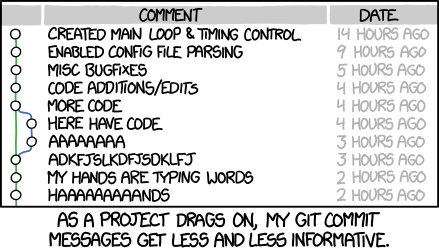
\includegraphics[width=0.45\textwidth]{xkcd-2}
        \end{center}
    \end{multicols}
\end{frame}

\begin{frame}[fragile]
    \frametitle{The Commit Message (Example)}

    \begin{lcverbatim}
Summarize changes in around 50 characters or less

More detailed explanatory text, if necessary. Wrap it to about 72
characters or so. In some contexts, the first line is treated as the
subject of the commit and the rest of the text as the body. The
blank line separating the summary from the body is critical (unless
you omit the body entirely); various tools like `log', `shortlog'
and `rebase' can get confused if you run the two together.

Explain the problem that this commit is solving. Focus on why you
are making this change as opposed to how (the code explains that).
Are there side effects or other unintuitive consequences of this
change? Here's the place to explain them.

Further paragraphs come after blank lines.

 - Bullet points are okay, too

 - Typically a hyphen or asterisk is used for the bullet, preceded
   by a single space, with blank lines in between, but conventions
   vary here
    \end{lcverbatim}
\end{frame}

\hugeslide{Demo}


\begin{frame}
    \frametitle{\shellcmd{Git}ting Better}

    Some more advanced commands to make your job easier.

    \begin{itemize}
        \item The wildcard \shellcmd{*} expands to whatever can fit a certain pattern.
        \begin{itemize}
            \item \shellcmd{git add *.cpp} stages all files with a \shellcmd{cpp} extension.
            \item \shellcmd{git add damon.*} add all document types with the name of \texttt{damon}, whether it be \shellcmd{cpp}, \shellcmd{txt}, or (unfortunately) \shellcmd{jpg}.
        \end{itemize}

        \item \shellcmd{git add -A} stages new, modified, and removed files.
        \item \shellcmd{git commit -m ``<msg>''} commits with the commit message \texttt{<msg>}. \textbf{Only use if you absolutely know what you're doing.}
    \end{itemize}
\end{frame}

\begin{frame}[t]
    \frametitle{Branching \presentcount{branching}}

    Branching is what allows for multiple people to work on multiple parts of the project.

    \vfill
    \begin{center}
        \begin{tikzpicture}
            \draw (0,0) circle [radius=0.3] node {a};
            \draw (1,0) circle [radius=0.3] node {b};
            \draw (2,0) circle [radius=0.3] node {c};
            \draw (5,0) circle [radius=0.3] node {d};
            \draw (8,0) circle [radius=0.3] node {e};


            \draw (3,1) circle [radius=0.3] node {d\textsubscript{1}};
            \draw (4,1) circle [radius=0.3] node {e\textsubscript{1}};

            \draw (3,-1) circle [radius=0.3] node {d\textsubscript{2}};
            \draw (4,-1) circle [radius=0.3] node {e\textsubscript{2}};
            \draw (6,-1) circle [radius=0.3] node {f\textsubscript{2}};
            \draw (7,-1) circle [radius=0.3] node {g\textsubscript{2}};

            \draw[thick,->] (0.3,0) -- (.7,0);
            \draw[thick,->] (1.3,0) -- (1.7,0);
            \draw[thick,->] (2.3,0) -- (4.7,0);
            \draw[thick,->] (5.3,0) -- (7.7,0);

            \draw[thick,->] (2.3,0) -- (2.7,1);
            \draw[thick,->] (3.3,1) -- (3.7,1);
            \draw[thick,->] (4.3,1) -- (4.7,0);

            \draw[thick,->] (2.3,0) -- (2.7,-1);
            \draw[thick,->] (3.3,-1) -- (3.7,-1);
            \draw[thick,->] (4.3,-1) -- (5.7,-1);
            \draw[thick,->] (6.3,-1) -- (6.7,-1);
            \draw[thick,->] (7.3,-1) -- (7.7,0);
        \end{tikzpicture}
    \end{center}
    \vfill

    So $D_1 \cdots E_1$ could be a bug fixing branch while $D_2 \cdots G_2$ could be a feature branch.
\end{frame}

\begin{frame}
	\frametitle{Branching \presentcount{branching}}
	\only<1>{\shellcmd{git checkout -b new-branch}}
	\only<2>{\shellcmd{git commit -m ``d''}}

    \vfill
	\centering
	\begin{tikzpicture}[->,>=stealth',shorten >=1pt,auto,node distance=2cm,
		semithick]
		\tikzstyle{every state}=[node distance=1.5cm]

		\node[state]   (A)  {a};

		\node[state] (B) [below of=A] {b};
		\path (A) edge (B);

		\node[state] (C) [below of=B] {c};
		\path (B) edge (C);

		\only<2->{%
			\node[state] (D) [below of=C] {d};
			\path (C) edge (D);
		}

		\node[draw=none] (M) [above left= 0.05cm and 1cm of C] {master};
		\path(M) edge (C);

		\only<1>{%
			\node[draw=none] (N) [left of=C] {new-branch};
			\path (N) edge (C);
		}
		\only<2>{%
			\node[draw=none] (N) [left of=D] {new-branch};
			\path (N) edge (D);
		}
	\end{tikzpicture}
\end{frame}

\begin{frame}
	\frametitle{Branching \presentcount{branching}}

	\only<2>{\shellcmd{git checkout master}}
	\only<3>{\shellcmd{git checkout -b another}}
	\only<4>{\shellcmd{git commit -m ``e''}}

    \vfill
	\centering
	\begin{tikzpicture}[->,>=stealth',shorten >=1pt,auto,node distance=2cm,
		semithick]
		\tikzstyle{every state}=[node distance=1.5cm]

		\node[state]   (A)  {a};

		\node[state] (B) [below of=A] {b};
		\path (A) edge (B);

		\node[state] (C) [below of=B] {c};
		\path (B) edge (C);

		\only<1-3>{%
		\node[state] (D) [below of=C] {d};
	}
	\only<4->{%
		\node[state] (D) [below left= 1.4cm of C] {d};
	}
		\path (C) edge (D);

		\only<4->{%
			\node[state] (E) [below right=1.4cm of C] {e};
			\path (C) edge (E);
		}

		\node[draw=none] (M) [above left= 0.05cm and 1cm of C] {master};
		\path(M) edge (C);

		\node[draw=none] (N) [left of=D] {new-branch};
		\path (N) edge (D);

		\only<1>{%
			\node[draw=none] (H) [right of=D] {\shellcmd{HEAD}};
			\path (H) edge (D);
		}
		\only<2-3>{%
			\node[draw=none] (H) [right of=C] {\shellcmd{HEAD}};
			\path (H) edge (C);
		}
		\only<4>{%
			\node[draw=none] (H) [right of=E] {\shellcmd{HEAD}};
			\path (H) edge (E);
		}

		\only<3>{%
			\node[draw=none] (Z) [left of=C] {another};
			\path (Z) edge (C);
		}
		\only<4>{%
			\node[draw=none] (Z) [left of=E] {another};
			\path (Z) edge (E);
		}
	\end{tikzpicture}
\end{frame}

\begin{frame}
    \frametitle{Merging \presentcount{merging}}
	\only<1-3>{\shellcmd{git merge new-branch}}
	\only<4>{\shellcmd{git merge master}\\ \shellcmd{Nothing to do!} \vspace{-1.2em}}
	\only<5>{\shellcmd{git checkout master}}
	\only<6>{\shellcmd{git merge another}}

	% \vspace{-1.2em}
    \vfill

    \centering
	\begin{tikzpicture}[->,>=stealth',shorten >=1pt,auto,node distance=2cm,
		semithick]
		\tikzstyle{every state}=[node distance=1.5cm]
		\node[state]   (A)  {a};

		\node[state] (B) [below of=A] {b};
		\path (A) edge (B);

		\node[state] (C) [below of=B] {c};
		\path (B) edge (C);

		\node[state] (D) [below left= 1.4cm of C] {d};
		\path (C) edge (D);

		\node[state] (E) [below right=1.4cm of C] {e};
		\path (C) edge (E);

		\only<2->{%
			\node[state] (Y) [below left=1.4cm of E] {d+e};
			\path (E) edge (Y)
						(D) edge (Y);
		}

		\only<1-5>{%
			\node[draw=none] (M) [above left= 0.05cm and 1cm of C] {master};
			\path(M) edge (C);
		}

		\only<6>{%
			\node[draw=none] (M) [above left= 0.05cm and 1cm of Y] {master};
			\path(M) edge (Y);
		}

		\node[draw=none] (N) [left of=D] {new-branch};
		\path (N) edge (D);


		\only<1>{%
			\node[draw=none] (H) [right of=E] {\shellcmd{HEAD}};
			\path (H) edge (E);
		}

		\only<1>{%
			\node[draw=none] (Z) [left of=E] {another};
			\path (Z) edge (E);
		}

		\only<3-4,6>{%
			\node[draw=none] (H) [right of=Y] {\shellcmd{HEAD}};
			\path (H) edge (Y);
		}

		\only<3->{%
			\node[draw=none] (Z) [left of=Y] {another};
			\path (Z) edge (Y);
		}

		\only<5>{%
			\node[draw=none] (H) [right of=C] {\shellcmd{HEAD}};
			\path (H) edge (C);
		}
	\end{tikzpicture}
\end{frame}

\begin{frame}
    \frametitle{Merging \presentcount{merging}}

    When working with larger repositories, you might not necessarily have rights to arbitrarily merge --- you have to create a \textit{merge request}. A merge request allows for someone to review the changes being made to the master branch. \textit{Because merge requests are different per hosting service, this will be shown in the demo.}
\end{frame}

\begin{frame}[fragile]
    \frametitle{Merge Conflicts \presentcount{conflicts}}
    On occasion, you might run into a merge conflict. These arise when you modify two parts of a shared code-base. For instance, an error message could appear like so:
    \begin{lcverbatim}
    Auto-merging the-files(s).txt
    CONFLICT (content): Merge conflict in the-file(s).txt
    Automatic merge failed; fix conflicts and then commit the result.
    \end{lcverbatim}

    Upon inspection, you should find something along the lines of:

    \begin{lcverbatim}
    <<<<<<< HEAD
    The current branch's contents
    =======
    The branch you're merging's contents
    >>>>>>> other-branch
    \end{lcverbatim}
\end{frame}

\begin{frame}
    \frametitle{Merge Conflicts \presentcount{conflicts}}

    There are many great ways to deal with merge conflicts!

    \begin{enumerate}
        \item Merge early, merge often. % Actually, there's only one. By merging smaller pieces, you get less merge conflicts. How can you achieve smaller merges? Having smaller branches
    \end{enumerate}

    \vfill
    \begin{center}
        \begin{tikzpicture}
            \draw (0,0) circle [radius=0.3] node {a};
            \draw (8,0) circle [radius=0.3] node {b};

            \draw[thick,->] (0.3,0) -- (.7,1);
            \draw (1,1) circle [radius=0.3] node {b\textsubscript{1}};
            \draw (7,1) circle [radius=0.3] node {c\textsubscript{2}};
            \draw[thick,->] (7.3,1) -- (7.7,0);

            \draw[thick,->] (0.3,0) -- (.7,-1);
            \draw (1,-1) circle [radius=0.3] node {c\textsubscript{2}};
            \draw (7,-1) circle [radius=0.3] node {c\textsubscript{2}};
            \draw[thick,->] (7.3,-1) -- (7.7,0);

            \draw[thick,->] (.3,0) -- (7.7,0) node[midway,fill=white] {\shellcmd{master}};
            \draw[thick,->] (1.3,1) -- (6.7,1) node[midway,fill=white] {Bug Fix Branch};
            \draw[thick,->] (1.3,-1) -- (6.7,-1) node[midway,fill=white] {Feature Branch};
        \end{tikzpicture}
    \end{center}
    \vfill
\end{frame}

\hugeslide{Demo}

\begin{frame}
    \frametitle{You Broke It --- Finding The Mistake}

    \begin{itemize}
        \item \shellcmd{git log} shows all previous commits. It has many useful parameters.
        \begin{itemize}
            \item \shellcmd{--stat} Shows statistics (deletions, insertions, files changed) for your files.
            \item \shellcmd{--pretty=oneline} A one line list of all your changes.
            \item \shellcmd{--graph} Shows a graph.
            \item \shellcmd{-p} Shows what are the changes to your code base.
        \end{itemize}

        \item \shellcmd{git diff} show the difference between the working directory and the last commit.
    \end{itemize}
\end{frame}

\begin{frame}
    \frametitle{You Broke It --- Fixing The Mistake}

    \begin{itemize}
        \item \shellcmd{git checkout COMMIT} Just as branches, looks at a previous commit.
        \item \shellcmd{git revert COMMIT} Generate a new commit that undoes all of the changes introduced in \shellcmd{COMMIT}, then apply it to the current branch.
        \item \shellcmd{git reset COMMIT} Move \shellcmd{head} to \shellcmd{commit} and reset the staging area to match. \textit{Leaves the working directory alone}.
        \item  \shellcmd{git reset --hard COMMIT} Move \shellcmd{head} to \shellcmd{commit} and reset the staging area to match. \textit{Destroys working direcory}. \textbf{Only use if you absolutely know what you're doing.}
    \end{itemize}
\end{frame}

\begin{frame}
    \frametitle{Working With Remotes}

    \begin{itemize}
		\item \shellcmd{git clone LOCATION} Makes a copy of a repository in the current directory --- you can set up SSH keys for Git/Gitlab or just use the url.
		\item \shellcmd{git push ORIGIN BRANCH} Pushes changes from your current branch to the remote branch it tracks.
		\item \shellcmd{git pull ORIGIN BRANCH} Pulls changes from the remote branch and merges them into your current branch.
	\end{itemize}
\end{frame}

\begin{frame}
    \frametitle{\shellcmd{Git}ting Better-est}

    If for the first time working on a repo, \shellcmd{git clone} the repo and \shellcmd{cd} into the directory. Then,

    \begin{enumerate}
        \item Pull any new changes with \shellcmd{git pull}.
        \item If starting a new feature or bug fix, create new branch with \shellcmd{git branch} (and switch to the branch with \shellcmd{git checkout}).
        \item Make your changes.
        \item Add your changes with either \shellcmd{git add FILE(s)} or \shellcmd{git add -A}\footnote{Only if you're sure you know what you're adding}.
        \item Commit your changes with \shellcmd{git commit}. Provide a \textbf{detailed} commit message.
        \item When feature/bug fix is finished, merge with either \shellcmd{git merge} or create a merge request. If there are merge conflicts, fix them.
        \item \shellcmd{git push} your changes.
    \end{enumerate}

\end{frame}


\begin{frame}
    \frametitle{In Closing}
    Special thanks to \href{http://web.mst.edu/~nmjxv3/}{Nathan Jarus} for ``lending'' me his \LaTeX{} tikz code for the branching, committing and merging section.

    % This only compiles with XeLaTeX
    \begin{description}
    \item [\faTwitter] \href{https://twitter.com/IllyaStarikov}{\nolinkurl{@IllyaStarikov}}
    \item [\faGithub]  \href{https://github.com/IllyaStarikov}{\nolinkurl{@IllyaStarikov}}
    \item [\faComment] \href{mailto:starikov@mst.edu}{\nolinkurl{starikov@mst.com}}
    \end{description}
\end{frame}

\end{document}
